% The Slide Definitions
%document
\documentclass[10pt]{beamer}
%theme
\usetheme{metropolis}
% packages
\usepackage{color}
\usepackage{listings}
\usepackage[ngerman]{babel}
\usepackage[utf8]{inputenc}
\usepackage{multicol}


% color definitions
\definecolor{mygreen}{rgb}{0,0.6,0}
\definecolor{mygray}{rgb}{0.5,0.5,0.5}
\definecolor{mymauve}{rgb}{0.58,0,0.82}

\lstset{
    backgroundcolor=\color{white},
    % choose the background color;
    % you must add \usepackage{color} or \usepackage{xcolor}
    basicstyle=\footnotesize\ttfamily,
    % the size of the fonts that are used for the code
    breakatwhitespace=false,
    % sets if automatic breaks should only happen at whitespace
    breaklines=true,                 % sets automatic line breaking
    captionpos=b,                    % sets the caption-position to bottom
    commentstyle=\color{mygreen},    % comment style
    % deletekeywords={...},
    % if you want to delete keywords from the given language
    extendedchars=true,
    % lets you use non-ASCII characters;
    % for 8-bits encodings only, does not work with UTF-8
    frame=single,                    % adds a frame around the code
    keepspaces=true,
    % keeps spaces in text,
    % useful for keeping indentation of code
    % (possibly needs columns=flexible)
    keywordstyle=\color{blue},       % keyword style
    % morekeywords={*,...},
    % if you want to add more keywords to the set
    numbers=left,
    % where to put the line-numbers; possible values are (none, left, right)
    numbersep=5pt,
    % how far the line-numbers are from the code
    numberstyle=\tiny\color{mygray},
    % the style that is used for the line-numbers
    rulecolor=\color{black},
    % if not set, the frame-color may be changed on line-breaks
    % within not-black text (e.g. comments (green here))
    stepnumber=1,
    % the step between two line-numbers.
    % If it's 1, each line will be numbered
    stringstyle=\color{mymauve},     % string literal style
    tabsize=4,                       % sets default tabsize to 4 spaces
    % show the filename of files included with \lstinputlisting;
    % also try caption instead of title
    language = Python,
	showspaces = false,
	showtabs = false,
	showstringspaces = false,
	escapechar = ,
}

\def\ContinueLineNumber{\lstset{firstnumber=last}}
\def\StartLineAt#1{\lstset{firstnumber=#1}}
\let\numberLineAt\StartLineAt



\newcommand{\codeline}[1]{
	\alert{\texttt{#1}}
}


% Author and Course information
% This Document contains the information about this course.

% Authors of the slides
\author{Claas de Boer, Tilman Hinnerichs}

% Name of the Course
\institute{Python-Grundlagen}

% Fancy Logo 
\titlegraphic{\hfill
\includegraphics[height=1.25cm]{../images/fsr_logo_cropped}}

% Custom Bindings
% \newcommand{\codeline}[1]{
%	\alert{\texttt{#1}}
%}


% Presentation title
\title{Objektorientierung}
\date{\today}


\begin{document}

\maketitle

\begin{frame}{Gliederung}
    \setbeamertemplate{section in toc}[sections numbered]
    \tableofcontents
\end{frame}

% ---- Was ist Objektorientierung ----
\section{Was ist \glqq Objektorientierung\grqq?}

\begin{frame}{\glqq Objektorientierung\grqq}
    \begin{itemize}
        \item Software als interagierende \glqq Objekte\grqq
        \item Objekte haben 
        \begin{itemize}
            \item Eigenschaften (\textbf{Attribute})
            \item Verhalten (\textbf{Methoden})
        \end{itemize}
    \end{itemize}
\end{frame}
\begin{frame}{Wozu?}
    \begin{itemize}
        \item \glqq intuitiver\grqq Entwurf
        \item Gruppierung von Daten und Verhalten $\rightarrow$ Klasse 
        \item Organisation großer Softwaresysteme
        \item $\rightarrow$ In Python grundlegend verankert
    \end{itemize}
\end{frame}
\begin{frame}{Beispiel}
    \texttt{random.randInt(min, max)} + Variablen $\rightarrow$ Objekt \glqq Würfel\grqq \begin{itemize}
        \item Attribute: \texttt{seiten}
        \item Methoden: \texttt{wuerfeln() -> int}
    \end{itemize}
    \begin{center}
        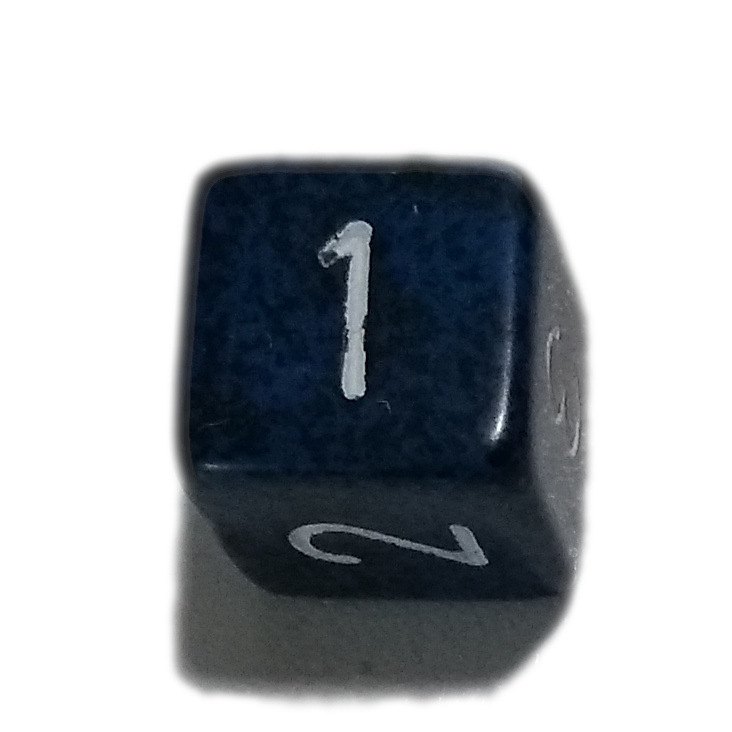
\includegraphics[width=0.5\textwidth]{d6.jpg}
    \end{center}
\end{frame}
\begin{frame}{Klassen}
    \begin{itemize}
        \item Oft mehrere Objekte einer Art gleich $\rightarrow$ Klassen
        \item Attribute, Methoden bei allen Objekten einer Klasse gleich
        \item Objekt ist \textbf{Instanz} einer Klasse
    \end{itemize}
    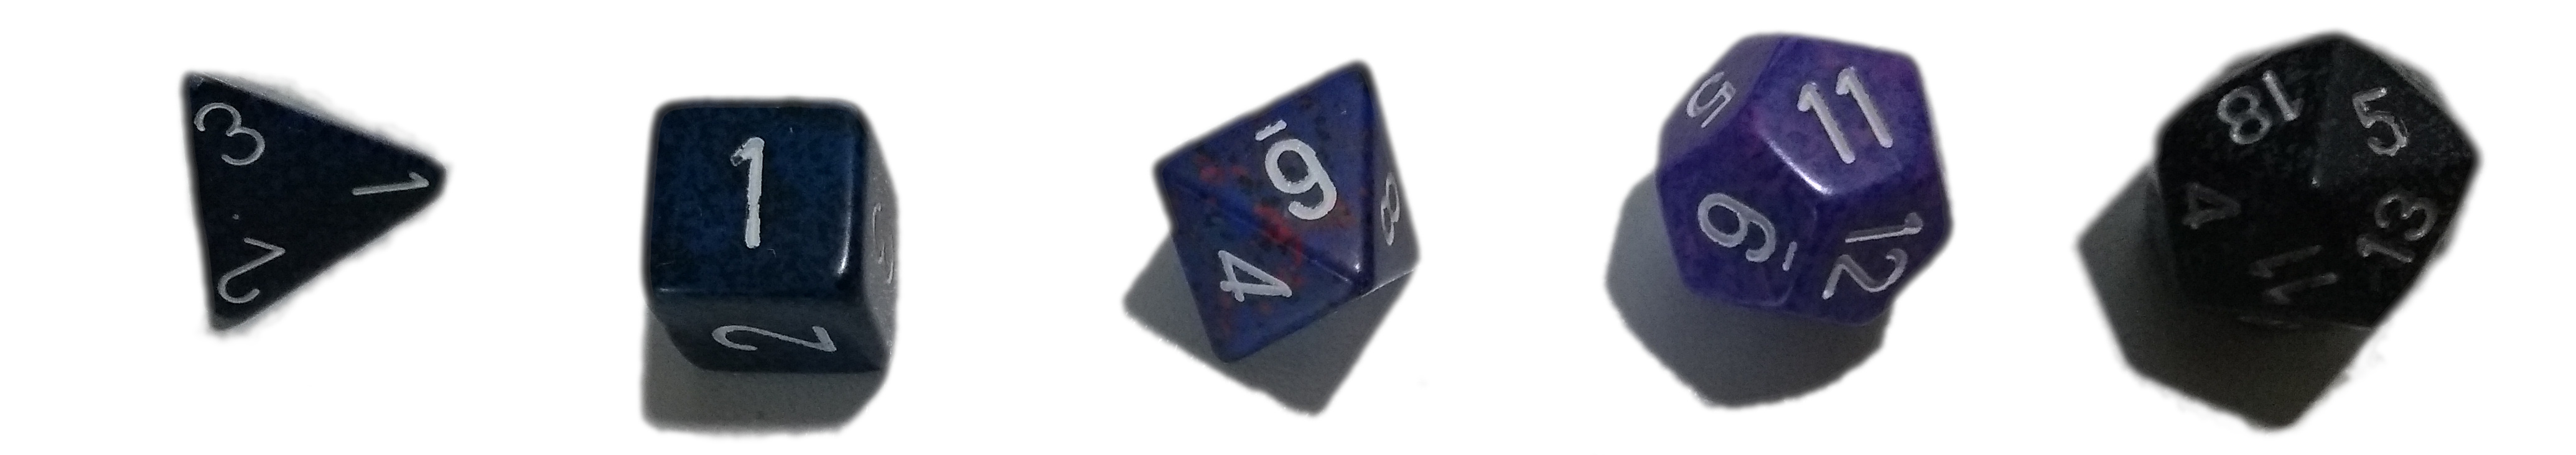
\includegraphics[width=\textwidth]{dice.jpg}
\end{frame}

% ----------------------- Objektorientierung in Python -----------------------

\section{Objektorientierung in Python}
\begin{frame}{Nutzen von Objekten}
    \begin{itemize}
        \item Wir kennen bereits Klassen und Objekte:
        \begin{itemize}
            \item \texttt{"Hello World"} ist \textbf{Instanz} von \texttt{str}
            \item \texttt{[1,2]} ist \textbf{Instanz} von \texttt{list}
        \end{itemize}
        \item Funktionen \texttt{sum([1,2,3])} $\leftrightarrow$ Methoden \texttt{[1,2,3].append(4)}!
    \end{itemize} 
\end{frame}

\begin{frame}[fragile]{Nutzen von Objekten}
    \begin{lstlisting}
# Erstellen eines neuen Objekts der Klasse list
l = [1,2,3]
# l ist tatsächlich Instanz von list
print(isinstance(l, list))

# Aufrufen der Methode append
l.append(4)
print (l) # Daten in der Liste wurden geaendert

print(len(l)) # len ist (eingebaute) Funktion, nicht Methode -> NICHT l.len!
    \end{lstlisting}
\end{frame}

\begin{frame}[fragile]{Eigene Klassen}
    \begin{lstlisting}
class Wuerfel:
    # VORSICHT: keine (Instanz-)Attribute hier!

    # spezielle Methode: Konstruktor. 
    # wird beim Erstellen einer Instanz aufgerufen
    def __init__(self, seiten):

        # neues Attribut "seiten" wird erzeugt.
        self.seiten = seiten

    # Methoden haben immer "self" als ersten Parameter
    # -> koennen so auf eigene Attribute zugreifen
    def wuerfeln(self):
        return random.randInt(1, self.seiten)
    \end{lstlisting}
\end{frame}

\begin{frame}[fragile]{Eigene Klassen}
    \begin{lstlisting}
        d6 = Wuerfel(6)
        d20 = Wuerfel(20)

        wert = d20.wuerfeln()
        print ("ich habe eine {} gewürfelt!".format(wert))
    \end{lstlisting}
\end{frame}

% --------------------- Aufgaben -------------------------

\section{Aufgaben}
\begin{frame}{Aufgaben}
    \begin{enumerate}
        \item Implementiere die Würfelklasse, erzeuge einen 20-seitigen Würfel und würfle. Falls du eine 20 würfelst, rufe laut "20"!
        \item Implementiere ein Würfelspiel, bei dem du und der Computer einmal würfeln. Wer die höhere Zahl würfelt, gewinnt!
        \item Schreibe eine Klasse \glqq Spieler\grqq, die einen Spieler bei diesem Würfelspiel darstellt. Welche Attribute und Methoden hat ein Spieler?
        \item Erweitere dein Würfelspiel, sodass zwei Spielerobjekte gegeneinander spielen.
        \item Zwei Spieler sind zu langweilig? Mit der Spielerklasse kannst du einfach mehr Spielerobjekte erzeugen. Erweitere dein Spiel, so dass beliebig viele Spieler spielen können (s. auch listen (letzte Stunde))
        \item Auch abstrakte Konzepte können als Klasse modelliert werden. Wie könnte man ein Würfelspiel mit mehreren Runden als Klasse darstellen?
    \end{enumerate}
\end{frame}

% ----------------------- Der Python Interpreter ------------------------------
% nothing to do from here on
\end{document}
